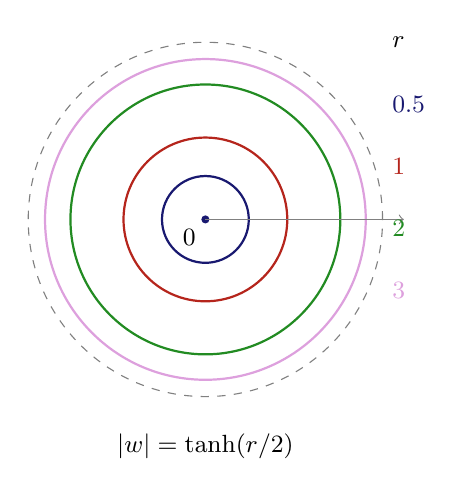
\begin{tikzpicture}[scale=2.25,font=\small]
\draw[gray,dashed] (0,0) circle (1);
\foreach \r/\col in {0.5/MidnightBlue,1/BrickRed,2/ForestGreen,3/Plum}{
  \pgfmathsetmacro{\rho}{(exp(\r)-1)/(exp(\r)+1)}
  \draw[\col,thick] (0,0) circle (\rho);
}
\fill[MidnightBlue] (0,0) circle (.65pt);
\draw[->,gray] (0,0)--(1.12,0);
\node[below left] at (0,0) {$0$};
\node[right] at (1,1) {$r$};
\node[MidnightBlue,right] at (1,.65) {$0.5$};
\node[BrickRed,right] at (1,.3) {$1$};
\node[ForestGreen,right] at (1,-.05) {$2$};
\node[Plum,right] at (1,-.4) {$3$};
\node at (0,-1.28) {$|w|=\tanh(r/2)$};
\end{tikzpicture}
